% Figure 2: the thesis in three panels, drawn from the cells of Table 1 and the memory table (pgfplots).
\begin{figure}[t]
\centering
\pgfplotsset{every axis/.style={font=\scriptsize, width=0.33\textwidth, height=0.26\textwidth,
  xtick={10,50,100,200}, xmode=log, log ticks with fixed point, xlabel={input frames $N$}, xlabel style={yshift=2pt},
  grid=major, grid style={black!10}, title style={font=\scriptsize, yshift=-3pt},
  legend style={font=\tiny, draw=none, fill=none, at={(0.5,-0.36)}, anchor=north, legend columns=-1, /tikz/every even column/.append style={column sep=4pt}},
  every axis plot/.append style={line width=0.9pt, mark size=1.4pt}}}
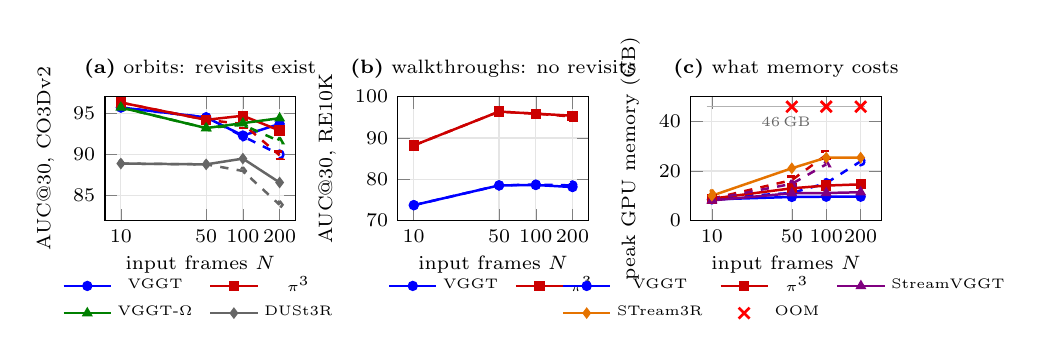
\begin{tikzpicture}
\begin{axis}[name=a, ylabel={AUC@30, CO3Dv2}, ymin=82, ymax=97, title={\textbf{(a)} orbits: revisits exist}, legend columns=2]
\addplot[blue, dashed, mark=o, forget plot] coordinates {(10,95.7)(50,94.5)(100,92.2)(200,90.0)};
\addplot[blue, mark=*] coordinates {(10,95.7)(50,94.5)(100,92.3)(200,93.7)};
\addplot[red!80!black, dashed, mark=square, forget plot] coordinates {(10,96.3)(50,94.2)(100,93.7)(200,89.9)};
\addplot[red!80!black, mark=square*] coordinates {(10,96.3)(50,94.2)(100,94.7)(200,92.9)};
\addplot[green!50!black, dashed, mark=triangle, forget plot] coordinates {(10,95.7)(50,93.2)(100,93.6)(200,91.6)};
\addplot[green!50!black, mark=triangle*] coordinates {(10,95.7)(50,93.2)(100,93.8)(200,94.4)};
\addplot[black!60, dashed, mark=diamond, forget plot] coordinates {(10,88.9)(50,88.8)(100,88.0)(200,83.9)};
\addplot[black!60, mark=diamond*] coordinates {(10,88.9)(50,88.8)(100,89.5)(200,86.6)};
\legend{VGGT, $\pi^3$, VGGT-$\Omega$, DUSt3R}
\end{axis}
\begin{axis}[name=b, at={(a.east)}, anchor=west, xshift=13mm, ylabel={AUC@30, RE10K}, ymin=70, ymax=100, title={\textbf{(b)} walkthroughs: no revisits}]
\addplot[blue, dashed, mark=o, forget plot] coordinates {(10,73.7)(50,78.5)(100,78.7)(200,78.5)};
\addplot[blue, mark=*] coordinates {(10,73.7)(50,78.5)(100,78.6)(200,78.1)};
\addplot[red!80!black, dashed, mark=square, forget plot] coordinates {(10,88.2)(50,96.4)(100,95.9)(200,95.2)};
\addplot[red!80!black, mark=square*] coordinates {(10,88.2)(50,96.4)(100,95.9)(200,95.4)};
\legend{VGGT, $\pi^3$}
\end{axis}
\begin{axis}[name=c, at={(b.east)}, anchor=west, xshift=13mm, ylabel={peak GPU memory (GB)}, ymin=0, ymax=50, title={\textbf{(c)} what memory costs}, legend columns=3]
\addplot[black!30, no marks, line width=0.6pt, forget plot] coordinates {(9,46)(220,46)} node[pos=0.5, below, font=\tiny, text=black!60] {46\,GB};
\addplot[blue, dashed, mark=o, forget plot] coordinates {(10,9.1)(50,11.1)(100,15.1)(200,23.9)};
\addplot[blue, mark=*] coordinates {(10,8.5)(50,9.5)(100,9.6)(200,9.6)};
\addplot[red!80!black, dashed, mark=square, forget plot] coordinates {(10,8.8)(50,16.3)(100,26.5)};
\addplot[red!80!black, mark=square*] coordinates {(10,8.8)(50,13.0)(100,14.1)(200,14.6)};
\addplot[violet, dashed, mark=triangle, forget plot] coordinates {(10,8.6)(50,14.8)(100,22.7)};
\addplot[violet, mark=triangle*] coordinates {(10,8.1)(50,11.0)(100,11.1)(200,11.4)};
\addplot[orange!90!black, dashed, mark=diamond, forget plot] coordinates {(10,10.9)};
\addplot[orange!90!black, mark=diamond*] coordinates {(10,10.0)(50,21.1)(100,25.4)(200,25.4)};
\addplot[only marks, mark=x, mark size=2.8pt, red, line width=1pt] coordinates {(200,46)(50,46)(100,46)};
\legend{VGGT, $\pi^3$, StreamVGGT, STream3R, OOM}
\end{axis}
\end{tikzpicture}
\vspace{-2mm}
\caption{\textbf{The thesis, measured} (cells of Tables~\ref{tab:pose} and~\ref{tab:memvsn}; dashed = raw or
native, solid = +\smr{}). (a) On CO3Dv2 orbits, raw chained windows lose accuracy with every added window;
the memory recovers most of it at $N{=}200$ and is identical to the backbone at $N{\le}50$, where no revisit
exists yet. (b) On RealEstate10K walkthroughs nothing is revisited, closures are ${\approx}0$, and the
memory correctly changes nothing --- the gain follows the mechanism. (c) Native inference pays for length in
VRAM (token cache, attention mask, alignment graph); three architectures hit the 46\,GB wall ($\times$), while
with \smr{} the cost is the window's and constant in $N$.}
\label{fig:results}
\end{figure}
